\chapter{Tecnologies Utilitzades}
\label{sec:tecnologies}

El programa que es vol desenvolupar durant el projecte ha d'utilitzar les següents tecnologies: 

\begin{enumerate}
	\item{Javascript com a llenguatge de programació.}
	\item{Node.js com a entorn d'execució del servidor.}
	\item{Websockets per a la comunicació entre el client i el servidor.}
	\item{HTML5,CSS i JQuery per a la capa de visualització del client.}
	\item{git com a programa de control de versions, utilitzant github per publicar el codi}
\end{enumerate}

\section{Perquè aquestes tecnologies?}

Abans de començar el projecte, quan en JM em va proposar de realitzar-lo em va dir que l'objectiu principal d'aquest projecte era provar, i a la vegada investigar el seu funcionament , noves tecnologies. Les que em va proposar són les següents: 
\begin{itemize}
	\item{Node.js}
	\item{Websockets}
	\item{HTML5, especialment l'objecte canvas}
\end{itemize}

Per la meva part desconeixia totalment l'existència de node.js i dels Websockets. Tot i tenia petits coneixements sobre HTML5, sabia que aquest no eren molt extensos i que eren necessari expandir-los.

El fet d'explorar noves tecnologies va ser molt motivador per mi, fins al punt de dir que ha estat una de les principals raons per decidir-m'hi per aquest projecte i no per un altre.  

Després d'explorar node.js vaig veure que el seu codi esta allotjat a github, i que la majoria dels mòduls que corren sobre ell també. Així em va semblar convenient allotjar tot el codi del projecte al mateix lloc. Github utilitza git com software de control de versions


\section{Javascript}

Javascript és un llenguatge script basat en el concepte de prototipus (herència per delegació), implementat originàriament per Netscape Communications Corporation l'any 1995, i que va derivar en L'estàndard ECMAScript. És conegut sobretot pel seu ús en pàgines web, però també s'utilitza en altres aplicacions.

En un principi, s'usava a pàgines web HTML, per realitzar feines i operacions al marc de l'aplicació client. Amb l'aparició de la Web 2.0, Javascript s'ha convertit en un veritable llenguatge de programació que aporta la potència de càlcul al navegador per augmentar l'usabilitat d'aplicacions web amb tècniques avançades com AJAX o JCC.

%TODO: (veure si cal) Explicar que es el DOM

\section{Node.js}

Node.js es un framework dissenyat per escriure aplicacions web altament escalables. Els programes s'escriuen amb Javascript. La seva estructura està basada en events i una entrada/sortida asíncrona. Aquest framework utilitza el motor de Javascript V8\footnote{\url{http://en.wikipedia.org/wiki/V8_JavaScript_engine}}. El motor V8 és de codi obert i està desenvolupat per Google, ja que aquest l'utilitza al seu navegador Google Chrome. Aquest motor millora el rendiment compilant el codi Javascript a codi natiu abans d'executar-lo.

La qualitat que fa diferent a node.js el seu funcionament està basat en events, i el codi s'executa en un sol thread/process. Això, provoca que els projectes que utilitzin aquest framework requereixin d'una programació diferent a la tradicional, asíncrona en comptes de seqüencial. 

\subsection{Codi Asíncron}

El fet de que el codi s'executi de forma asíncrona, implica que el programa pot realitzar diferents tasques mentre espera que el sistema realitzi alguna altra tasca. Això vol dir que el programa pot seguir realitzant tasques mentre espera que es realitzi una consulta a la base de dades, que es llegeixi un fitxer des de disc, o que es rebin les dades d'un servidor extern. Així el programa s'estructura amb el que es coneix com a callbacks. Un callback es el codi que s'executara després d'haver realitzat alguna tasca. 

\begin{lstlisting}
fs.readFile(__dirname + '/someDir/someFile', 'utf8', function (err,data) {
  if (err) {
    return console.log(err);
  }
  console.log(data);
});
\end{lstlisting}

En aquest text es pot veure el codi necessari per a llegir un fitxer de disc. Així el que es fa es dir-li al sistema, llegeix el fitxer /someDir/someFile. Una vegada hagis acabat executa la funció que es passa a l'ultim paràmetre. Amb això aconseguim que mentre el proces estigui llegint el fitxer nosaltres puguem seguir fent càlculs, i que quan s'hagi acabat la lectura del fitxer puguem fer amb ell el que creguem convenient. 

El procesament asíncron és fa gracies als anomenats events, que s'encarreguen d'executar codi font quan s'ha produit alguna cosa. A més a més, node ens permet crear events personalitzats i fer que s'executi el nostre codi cada vegada que es produeix un event. Els events han estat utilitzats en gran part del desenvolupament del projecte. 
%TODO: Fer un apartat per comparar el codi asincron amb el codi asincron.
%TODO:
%Tot i que node.js es un framwork bastant inusual, les primeres impresions ell van ser magnífiques. 
%Primer de tot utilitza codi Javascript per a crear servidors, quan tots els meus coneixements eren per executar codi Javascript en l'entorn de client. La segona cosa que em va sorprendre molt de node.js va ser que aquest sigui un entorn d'execució de programés asíncrons. 

\section{Websockets}
\label{sec:websockets}

WebSocket és una tecnologia que proporciona un canal de comunicació bidireccional i full-duplex sobre un únic socket TCP. Està dissenyada per ser utilitzada en navegadors i servidors web, però pot utilitzar-se per qualsevol aplicació client/servidor. La API de WebSocket s'està normalitzant pel W3C\footnote{World Wide Web Consortium}, i el protocol WebSocket, a la vegada, s'està normalitzant per l'IETF\footnote{Internet Engineering Task Force}. Normalment, per temes de seguretat, els administradors de xarxes bloquegen les connexions als ports diferents del port 80, així els WebSockets pretenen solucionar aquest problema, aportant una tecnologia que proporcioni una funcionalitat similar a la que s'obté obrint diferents connexions en diferents ports però multiplexant els diferents serveis de a través d'un únic port TCP.

\section{HTML5}

HTML representa les sigles de \emph{Hyper Text Markup Language}, que en català signifiquen "llenguatge de marcat d'hipertext". És un llenguatge de marcat que deriva de l'SGML dissenyat per estructurar textos i relacionar-los en forma d'hipertext. Gràcies a Internet i als navegadors web, s'ha convertit en un dels formats més populars que existeixen per a la construcció de documents per a la web. 

HTML5 és la última versió de HTML. Aquesta última versió proporciona noves marques per poder estructurar els documents d'una forma més semàntica. A més a més proporciona noves etiquetes per poder etiquetar contingut multimèdia, ja sigui àudio o vídeo. També afegeix una nova etiqueta "canvas" que permet la representació dinàmica de formes 2D i imatges a través de llenguatge Javascript. 

\subsection{L'objecte canvas}

El fet de que l'objecte canvas utilitzi el llenguatge permet realitzar dibuixos amb interacció de l'usuari. Això ens permet deixar que l'usuari dibuixi amb el click del seu ratolí, o que es crein un dibuix después de que l'usuari seleccioni alguna opció. Així, l'objecte canvas ens permet realtizar animacions de qualitat igualable a la que es poden obtenir amb el software d'animació Flash\footnote{\url{http://www.adobe.com/es/products/flash.html}}, evitant la necesitat de que l'usuari hagi d'instal·lar un connector per a reproduïr-los. 

L'objecte canvas és un estándar per la web, se'n poden trobar les especificacions\footnote{\url{http://www.w3.org/TR/html5/the-canvas-element.html}} a la pàgina del W3C\footnote{World Wide Web Consorcium: \url{http://www.w3.org/}}

Així dins d'un objecte canvas podem realitzar les següents animacions: 

\begin{itemize}
\item{Escalar el dibuix.}
\item{Girar el dibuix.}
\item{Dibuixar una imatge.}
\item{Escriure textos.}
\item{Dibuixar lines rectes.}
\item{Dibuixar rectangles.}
\item{Dibuixar arcs.}
\item{Composar objectes.}
\item{Afegir sombres als objectes.}
\item{Crear degradats.}
\end{itemize}

Totes aquests metodes ens permeten crear tot tipus de dibuixos i animacions.

\newpage

\subsubsection{Alguns exemples de l'objecte canvas}

En l'exemple a continuació podem veure el codi necesari per a pintar dos rectangles de dos colors un damunt de l'altre. Com podeu veure es tracta de codi HTML i Javascript.  

\begin{lstlisting}[language=html]
<html>
<head>
<script language="Javascript">
function draw() {
    var canvas = document.getElementById("canvas");
    if (canvas.getContext) {
        var ctx = canvas.getContext("2d");
        ctx.fillStyle = "rgb(40,0,0)";
        ctx.fillRect (20, 20, 65, 60);
        ctx.fillStyle = "rgba(0, 0, 160, 0.5)";
        ctx.fillRect (40, 40, 65, 60);
    }
}
</script>
</head>
<body onLoad="draw();">
<canvas id="canvas" width="150" height="150">No teniu un navegador amb suport per visualitzar elements canvias.</canvas>
</body>
</html>
\end{lstlisting}

Com podeu veure a la línea 17 el que fem es declarar un objecte canvas de 150px d'ample per 150 pixels de l'alt. Aquest es l'espai on dibuixarem el nostre dibuix. El text que està contingut dins de l'etiqueta canvas serà el que es mostrarà pels navegadors que no tinguin suport per l'etiqueta canvas. 

Una vegada carregada la pàgina el que fem es cridar la funció draw(), que és l'encarregada de realitzar el dibuix. D'aquesta funció en podem destacar la següent informació:

\begin{description}
\item[línies 6,7 i 8]{Encarregades d'obtenir el contexte en per realitzar els dibuixos, només en el cas de que això sigui suportat pel navegador de l'usuari.}
\item[línia 9]{Canvia el color de farciment per als pròxims dibuix.}
\item[línia 10]{Dibuixa un rectangle prenen com a inici les coordenades (20,20) del canvas, i d'una mida de 65x65.}
\item[línia 11]{Canvia el color de parciment. A més a més asigna una transparència del 50\% (quart paràmetre.}
\item[línia 12]{Dibuixa un rectangle prenen com a inici les coordenades (40,40) del canvas, i d'una mida de 65x65.}
\end{description}

A la figura \ref{fig:canvas-exemple-1} podeu veure el resultat del codi comentat anteriorment. 

\begin{figure}[htbp]
\centering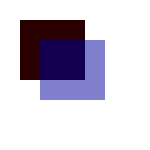
\includegraphics{img/canvas_example1.png}
\caption{Dibuix de dos rectangles superposats amb canvas.}
\label{fig:canvas-exemple-1}
\end{figure} 

L'exemple a continuació s'ha extret\footnote{El codi ha estat simplificat per simplificar la seva comprensió.} de la pàgina html5canvastutorials.com\footnote{\url{http://www.html5canvastutorials.com/advanced/html5-canvas-linear-motion-animation/}}. En aquest exemple es descriurà com animar un objecte que s'ha creat dins del canvas, en concret es farà moure un rectangle desde la part esquerra del canvas fins a la seva part dreta. A la mateixa pàgina podeu trobar una demostració de com funciona el codi que es detalla a continuació.  

\begin{lstlisting}
window.requestAnimFrame = (function(callback){
    window.setTimeout(callback, 1000 / 60);
})();
 
function animate(lastTime, myRectangle){
    var canvas = document.getElementById("myCanvas");
    var context = canvas.getContext("2d");
 
    // update
    var date = new Date();
    var time = date.getTime();
    var timeDiff = time - lastTime;
    var linearSpeed = 100; // pixels / second
    var linearDistEachFrame = linearSpeed * timeDiff / 1000;
    var currentX = myRectangle.x;
 
    if (currentX < canvas.width - myRectangle.width - myRectangle.borderWidth / 2) {
        var newX = currentX + linearDistEachFrame;
        myRectangle.x = newX;
    }
    lastTime = time;
 
    // clear
    context.clearRect(0, 0, canvas.width, canvas.height);
 
    // draw
    context.beginPath();
    context.rect(myRectangle.x, myRectangle.y, myRectangle.width, myRectangle.height);
 
    context.fillStyle = "#8ED6FF";
    context.fill();
    context.lineWidth = myRectangle.borderWidth;
    context.strokeStyle = "black";
    context.stroke();
 
    // request new frame
    requestAnimFrame(function(){
        animate(lastTime, myRectangle);
    });
}
 
window.onload = function(){
    var myRectangle = {
        x: 0,
        y: 50,
        width: 100,
        height: 50,
        borderWidth: 5
    };
 
    var date = new Date();
    var time = date.getTime();
    animate(time, myRectangle);
};
\end{lstlisting}

En aquestes exemple es creen tres funcions que són les encarregades de realitzar la animació. L'objectiu de cada funció és el següent:

\begin{description}
    \item[requestAnimFrame]{ S'encarregar de programar l'execcució del pròxim pas de l'animació}
    \item[animate]{ Es l'encarregada de realitzara cada un dels pasos de l'animació.}
    \item[window.onload] { Es la funció encarregada d'iniciar l'animació. Com es pot observar l'unic que fa es inicialitzar les variables i cridar a la funció animate per a que dibuixi el primer frame de l'animació.}
\end{description}

De la funció animate (la que s'encarrega de pintar cada un dels frames de l'animació) cal destacar les següents línies:

\begin{description}
    \item[línies 12-22] {Encarregades de calcular el temps que ha pasat desde l'ultima execució del codi, per poder saber el nombre de pixels que s'ha de moure l'objecte, tenint en compte que s'utilitza la variable linearSpeed per determinar el nombre de pixels per segons que ha d'abansar l'objecte.}
    \item[línies 25-26] {Netejar tot el conjunt de l'objecte canvas per tal d'esborrar els possibles frames anteriors.}
    \item[línies 28-36] {Encarregades de dibuixar el rectangle a la posició que li toca per al frame actual.}
    \item[línies 38-41] {Crida a la funció requestAnimFrame per programar l'execució del proxim frame.}
\end{description} 


\section{CSS}

CSS representa les sigles de \emph{Cascading Style Sheets}, que en catalpa signifiquen "Fulls d'estil en cascada". és un llenguatge de fulls d'estil utilitzat per descriure la semàntica de presentació (l'aspecte i format) d'un document escrit en un llenguatge de marques. La seva aplicació més comuna és dissenyar pàgines web escrites en HTML i XHTML, però el llenguatge també pot ser aplicat a qualsevol classe de document XML, incloent-hi SVG i XUL.

El principal objectiu de CSS es permetre la separació del contingut d'un document escrit amb un llenguatge de marques de la seva presentació. Aquesta separació permet que múltiple pàgines comparteixin un format comú i també que un mateix document de marcatge es pugui mostrar en diferents formats. 

CSS defineix regles d'estil per a cada element, on s'especifica com es mostrarà cada element. Així també definies un esquema de prioritat per determinar quines regles d'estil s'apliquen si més d'una regla esta associada amb un element en particular. Aquestes característiques han permès que avui en dia sigui el llenguatge més utilitzat a l'hora de definir l'aspecte i el format d'una pàgina web. 

\section{JQuery}

JQuery és una llibreria de Javascript, creada inicial ment per John Resig, que permet simplificar la forma d'interactuar amb els documents HTML, manipular l'arbre DOM, interactuar amb els events, desenvolupar animacions y afegir interacció dinàmica a pàgines web. 

JQuery es software de codi obert, llicenciat sota les llicències MIT y LGPLv2, permeten ser usada tan a projectes lliures com a projectes privatius. 

\section{Git i Github}

Git es un sistema de control de versions \footnote{\url{http://es.wikipedia.org/wiki/Control_de_versiones}} dissenyat per Linus Trovalds, creador de Linux. Git té les següents característiques principals: 

\begin{description}
    \item[Suport per desenvolupament no lineal] Git està dissenyat per tal de proporcionar una interfície ràpida per a crear branques i mesclar-les.
    \item[Distribuït] Cada usuari té un repositori propi. Aquests respositoris poden ser fusionats amb respositoris d'altres usuaris.
    \item[Compatibilitat amb protocols existents] Els respositoris poden ser publicats mitjançant protocols HTTP,FTP,Rsync i fins i tot un protocol propi.
    \item[Eficient per grans projectes] Git es ràpid i escalable. A més a més no es fa més lent a mesura que la història del projecte es fa gran, com passa amb altres sistemes.
    \item[Portable] Funciona tan en sistemes Linux,Unix,MAC i Windows.
\end{description}

Github un servei de d'allotjament de codi per a repositoris Git. A part d'allotjar el teu propi repositori ofereix altres serveis com poden ser Gist\footnote{\url{https://gist.github.com/}} (per a compartir petits trossos de codi), una wiki per projecte, allotjament de pàgines web i un petit gestió d'incidències molt flexible. A data 16/12/2011 compta amb 1,184,001 persones i allotja 3,448,813 repositoris.

Github ofereix il·limitats repositoris de forma gratuïta sempre que el seu codi sigui públic. A més a més ofereix repositoris privats per un petit preu mensual. 

\section{Mocha i jscoverage}

Mocha\footnote{\url{http://visionmedia.github.com/mocha/}} és una llibreria que s'encarrega d'executar jocs de prova i que funciona sobre el framework node. Aquesta llibrería s'encarrega de detectar quins dels nostres testos están fallant i reportar-nos els errors a través de diferents formats. Una de les aplicacions més interessant de Mocha és la generació de informes de coverage. Un informe de coverage ens permet visualitzar quines són línies de codi de l'aplicació són executades per un joc de proves i quines no. Per a la genereació d'aquest informes es requereix tenir instal·lada la llibreria jscoverage\footnote{\url{http://siliconforks.com/jscoverage/}}. 



